% Loss ratio across VLM variants on medical and UAV.
% Higher = stronger attack.
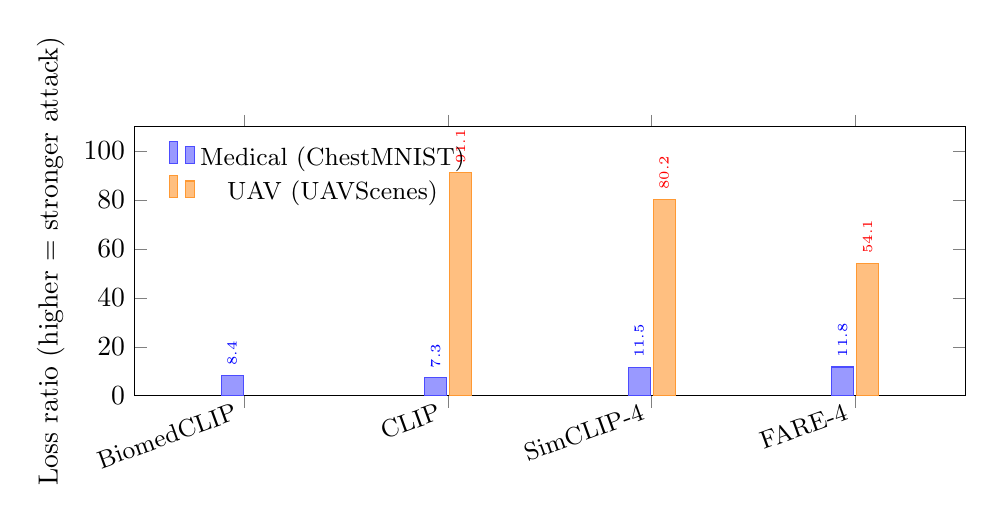
\begin{tikzpicture}
\begin{axis}[
    width=\columnwidth,
    height=5cm,
    ybar=1pt,
    bar width=8pt,
    enlarge x limits=0.18,
    ylabel={Loss ratio (higher = stronger attack)},
    symbolic x coords={BiomedCLIP, CLIP, SimCLIP-4, FARE-4},
    xtick=data,
    xticklabel style={font=\small, rotate=20, anchor=east},
    ytick={0,20,40,60,80,100},
    ymin=0, ymax=110,
    legend pos=north west,
    legend style={font=\small, draw=none, fill=none},
    nodes near coords={\pgfmathprintnumber[fixed,precision=1]{\pgfplotspointmeta}},
    nodes near coords style={font=\tiny, rotate=90, anchor=west},
    every node near coord/.append style={
        /pgf/number format/assume math mode=true
    },
]
\addplot+[fill=blue!40, draw=blue!70, /pgf/nan/.style={hide point=true}] coordinates {
    (BiomedCLIP, 8.39)
    (CLIP, 7.32)
    (SimCLIP-4, 11.46)
    (FARE-4, 11.75)
};
\addplot+[fill=orange!50, draw=orange!80] coordinates {
    (CLIP, 91.12)
    (SimCLIP-4, 80.20)
    (FARE-4, 54.11)
};
\legend{Medical (ChestMNIST), UAV (UAVScenes)}
\end{axis}
\end{tikzpicture}
